\section{On the number of types in sparse graph classes}\label{sec:types}

In this section we prove \Cref{thm:vc-density} and \Cref{thm:vc-density-lower-bound}.
	Recall that \Cref{thm:vc-density} provides upper bounds on the number of types in classes of graphs which are nowhere dense, 
	and stronger bounds for classes which have bounded expansion. 
	On the other hand, the complementary \Cref{thm:vc-density-lower-bound} shows that for subgraph-closed classes, in the absence of structural sparsity we cannot hope for such upper bounds.

\paragraph*{Upper bounds for sparse classes.}
We first prove \Cref{thm:vc-density}.
From now on we fix a formula  $\phi(\tup x,\tup y)$
with $\ell$ object variables

% For a graph $G$, a set of  vertices $A\subset V(G)$, and a tuple $\tup v\in V(G)^n$,
% denote
% \[\phi(A,\tup v)=\setof{\tup a \in A^m }{ G\models\phi(\tup a,\tup v)}.\]
% We call $\phi(A,\tup v)$ the \emph{$\phi$-type} of $\tup v$ \emph{over} $A$, and
% $A$ is sometimes called the \emph{parameter set}.
% For $W\subset V(G)$, denote
% \[S_\phi(A,W)=\setof{\tp^\phi_G(\bar v/A)}{ \tup v\in W^n}.\]
% Note that $S_\phi(A,W)$ is \emph{not} symmetric in $A$ and $W$.
% We write $S_\phi(A,G)$ as a shorthand for $S_\phi(A,V(G))$.
% The set $S_\phi(A,G)$ is therefore the set of all $\phi$-types of $n$-tuples
% of vertices of $G$ over the parameter set $A$.
We show  that if $\CCC$ is a nowhere dense class,
then for every $\varepsilon>0$ we have  $|S^\phi(G/A)|\le \Oof(|A|^{\ell+\varepsilon})$,
for all $G\in \CCC$ and $A\subset V(G)$,
 and 
if $\CCC$ is moreover of bounded expansion, then in fact $|S^\phi(G/A)|\le \Oof(|A|^\ell)$.


To prove~\cref{thm:vc-density},
we will first enlarge the set $A$ to a set $B$, called
an \emph{$r$-closure of $A$}, such 
that the connections of elements from $V(G)\setminus B$ 
towards $B$ are well controlled. This approach
was first used in Drange et al.~\cite{drange2016kernelization} in the context of classes of bounded expansion, 
and then for nowhere dense classes in Eickmeyer et al.~\cite{eickmeyer2016neighborhood}. 
We recall these notions.

Let $G$ be a graph and let $B\subseteq V(G)$ be a subset of vertices. For vertices $v\in B$ and $u\in V(G)$, a path $P$ connecting $u$ and $v$ is called {\em{$B$-avoiding}}
if all its vertices apart from~$v$ do not belong to $B$. For a positive integer $r$ and $u\in V(G)$, the {\em{$r$-projection}} of $u$ on $B$, denoted $M^G_r(u,B)$, is the set of all vertices $v\in B$ that
can be connected to $u$ by a $B$-avoiding path of length at most $r$. Note that for $u\in B$, we have $M^G_r(u,B)=\{b\}$.
Equivalently, $M^G_r(u,B)$ is the inclusion-minimal
subset of $B$ which $r$-separates $u$ from $B$.

%
%The {\em{$r$-projection profile}} of a vertex $u\in V(G)\setminus A$ on $A$ is a function $\rho^G_r[u,A]$ mapping vertices of
%$A$ to $\{0,1,\ldots,r,\infty\}$, defined as follows: for every $v\in A$, the value $\rho^G_r[u,A](v)$ is the length of a shortest $A$-avoiding path connecting $u$ and~$v$, and~$\infty$ in case this length
%is larger than $r$. 
%
% \begin{comment}
\begin{figure}[h!]
	\centering
		\includegraphics[scale=0.35,page=2]{pics}
	\caption{The  $r$-projection of $u$ on $B$
	(here $r=2$)
	is the minimal (inclusion-wise) set  $S\subset B$
	which $r$-separates $ u$ from $B$.
	}
	\label{fig:gaifman}
\end{figure}
% \end{comment}

% We define
% \[\projnum_r(G,B)=|\{M_r^G(u,B)\colon u\in V(G)\}|\]
%\quad\textrm{and}\quad \projprof_r(G,A)=|\{\rho_r^G[u,A]\colon %u\in V(G)\setminus A\}|\]
% to be the number of different $r$-projections on $B$.
We will use the following results from~\cite{drange2016kernelization,eickmeyer2016neighborhood}.
% and $r$-projection profiles realized on $B$, respectively. Clearly, it %holds that $\projnum_r(G,A)\leq \projprof_r(G,A)$.

\begin{lemma}[\cite{drange2016kernelization}]\label{lem:closure-be}
Let $\CCC$ be a class of bounded expansion. 
Then for every $r\in \N$ there is a constant $c\in \N$ such that for
every $G\in \CCC$ and $X\subseteq V(G)$ there exists a set $\cl_r(X)$, called an {\em{$r$-closure}} of $X$, with the following properties. 
\begin{enumerate}[(a)]
  \item $X\subseteq \cl_r(X)\subseteq V(G)$;
  \item $|\cl_r(X)|\leq c\cdot |X|$; 
  \item $|M_r^G(u,\cl_r(X))|\leq c$ for each $u\in V(G)$; and
  \item $|\setof{M_r^G(u,\cl_r(X))}{u\in V(G)}|\leq c\cdot |\cl_r(X)|$.
\end{enumerate}
\end{lemma}

\begin{lemma}[\cite{eickmeyer2016neighborhood}]\label{lem:closure-nd}
Let $\CCC$ be a nowhere dense class. 
Then for every $r\in\N$ and $\epsilon>0$ there is a 
constant $c\in\N$ such that for every $G\in \CCC$ and $X\subseteq V(G)$ there exists a set 
$\cl_r(X)$,  called an {\em{$r$-closure}} of $X$, 
with the following properties: 
\begin{enumerate}[(a)]
  \item $X\subseteq \cl_r(X)\subseteq V(G)$;
  \item $|\cl_r(X)|\leq c\cdot |X|^{1+\epsilon}$; 
  \item $|M_r^G(u,\cl_r(X))|\leq c\cdot |X|^{\epsilon}$ for each $u\in V(G)$; and
  \item $|\setof{M_r^G(u,\cl_r(X))}{u\in V(G)}|\leq c\cdot |\cl_r(X)|^{1+\epsilon}$.
\end{enumerate}
\end{lemma}

% \begin{lemma}[\cite{drange2016kernelization}]\label{lem:projection-complexity-be}
% Let $\CCC$ be a class of bounded expansion. Then for every $r\in \N$ there is
%   a constant $c\in\N$ such that for every graph $G\in \CCC$ and vertex subset $A\subseteq V(G)$,
%   it holds that $\projnum_r(G,A)\leq c\cdot |A|$.
% \end{lemma}
%
% \begin{lemma}[\cite{eickmeyer2016neighborhood}]\label{lem:projection-complexity-nd}
% Let $\CCC$ be a nowhere dense class. Then for every $r\in \N$ and $\epsilon>0$ there is
%   a constant $c\in \N$ such that for every graph $G\in \CCC$ and vertex subset $A\subseteq V(G)$,
%   it holds that $\projnum_r(G,A)\leq c\cdot |A|^{1+\epsilon}$.
% \end{lemma}
\begin{comment}
Figure~\ref{fig:closure} illustrates~\cref{lem:closure-nd}.
\begin{figure}[t]
	\centering
		\includegraphics[scale=0.35,page=3]{pics}
	\caption{An illustration of \Cref{lem:closure-nd}. The $r$-closure $B$ of $A$ has the following three properties:
(a) its size is  $\Oof(|A|^{1+\epsilon})$,
(b) it has at most $\Oof(|B|^{1+\epsilon})$ distinct $r$-projections,
(c) every $r$-projection has size $\Oof(|B|^\epsilon)$.
}
	\label{fig:closure}
\end{figure}
\end{comment}

We note that in~\cite{drange2016kernelization,eickmeyer2016neighborhood} projections on $B$ are defined only for vertices outside of $B$. 
However, adding singleton projections for vertices of $B$ to the definition only adds $|B|$ possible projections of size $1$ each, so this does not influence the validity of the above results.


\medskip
We  now prove~\cref{thm:vc-density}, whose statement we repeat for convenience. 
\setcounter{theorem}{2}
\begin{theorem}
Let $\CCC$ be a class of graphs and let $\phi(\tup x,\tup y)$ be a first-order formula with distinguished object variables $\bar x$ and parameter variables $\bar y$, and let $\ell=|\bar x|$. Then:
\begin{enumerate}[(1)]
\item If $\CCC$ is nowhere dense, then for every $\epsilon>0$ 
there exists a constant~$c$ such that for every $G\in \CCC$ and every nonempty
$A\subseteq V(G)$ the inequality $|S^\phi(G/A)|\leq c\cdot |A|^{\ell+\epsilon}$ holds.

\item If $\CCC$ has bounded expansion, then there exists a constant~$c$ such that for every $G\in \CCC$ and every nonempty $A\subseteq V(G)$ the inequality $|S^\phi(G/A)|\leq c\cdot |A|^\ell$ holds.
\end{enumerate}
\end{theorem}


\begin{proof}
	% We only discuss the proof in the case of a nowhere dense class $\cal C$; the case of bounded expansion classes  is analogous, and can be obtained from the proof below
% 	by replacing all the values $\epsilon,\delta,\epsilon_1,\epsilon_2,\epsilon_3$ below by $0$.
%
	
% We use the following notation.\newcommand{\Uof}{{\cal U}}
%  % as defined by Hardy and Littlewood, and later used by Landau (and later redefined by Knuth), i.e.,
% We write $f(n)=\Uof(g(n))$ to denote that $f(n)$ is \emph{unbounded} in terms of $g(n)$, i.e., for every fixed number $c>0$, there are infinitely many values $n$ such that $|f(n)|>c\cdot |g(n)|$.
%  In other words, $f(n)=\Uof(g(n))$ is the negation of $f(n)=\Oof(g(n))$. Abusing this notation slightly,
%  in the following proof by contradiction
%  we will say e.g.  ``there is an  $n$
%  such that $f(n)=\Uof(g(n))$'', meaning that
%  there is an $n$ such that
%   $|f(n)|>c\cdot |g(n)|$, where the constant $c$ is chosen sufficiently large so that the following contradiction will be obtained.
 
	
  Fix a first order formula $\phi(\bar x,\bar y)$, where $\bar x$ is the distinguished $\ell$-tuple of object variables.
    By \emph{tuples} below we refer to tuples of length $\ell$.
	   Fix a real $\epsilon$ which is positive if $\cal C$
	   is nowhere dense and equal to $0$ if $\cal C$ has bounded expansion.	   
	   We show that $|S^\phi(G/A)|$ is $\Oof(|A|^{\ell+\epsilon})$.
	   \medskip
	   
	   
	   
In the proof below, $d$ denotes a positive integer 
depending on ${\cal C},\ell,\phi$ only (and not on $G, A$ and $\epsilon$), which will be specified later.
Similarly, $\delta,\epsilon_1,\epsilon_2,\epsilon_3$ denote  reals which 
will be specified later.
These values, as well as the constants hidden in the $\Oof$ notation, depend
 on $\epsilon,\cal C, \ell$ and $\phi$, but not on $G$ and $A$.
 In the case of nowhere dense classes the  parameters $\delta,\epsilon_1,\epsilon_2,\epsilon_3$ are positive. The case of bounded expansion classes is the simpler, degenerate  case, where $\epsilon,\delta,\epsilon_1,\epsilon_2,\epsilon_3$  are taken to be $0$. To focus attention, we consider only the nowhere dense case below.
 
The parameters $\delta$ and $\epsilon_1$ are chosen so that 
%
%
%  $(1+\delta)^2<\frac{\ell+\epsilon}{\ell+d}$.
%  In particular, $\delta d+(\delta+1)\ell\le
%  (\delta+1)(d+\ell)<
%  \frac{\ell+\epsilon}{1+d}$.
% The parameter $\epsilon_1$ is such that
% $\delta d+(\delta+1)\ell<\ell+\epsilon_1<\frac{\ell+\epsilon}{1+d}$.
%  In particular,
%  $\delta\ell\le \delta(d+\ell)\le $
% The parameter $\epsilon_1$ will be such that $\cdots$
% 	% $1+\delta<1+\epsilon_1<\frac{1+\epsilon/\ell}{1+\delta}$.
% 	In particular,
	 $ (\ell+\epsilon_1)(1+\delta)%\le 	 \ell(1+\epsilon_1)(1+\delta) 
	 \le
	 \ell+\epsilon$ and $\epsilon_1>\delta(d+\ell)\ge \delta\ell$.
	 It is easy to check\footnote{Pick $\delta$ so that 
	 $\delta((1+\delta)(d+\ell)+\ell)<\epsilon$. Then $\delta(d+\ell)+\ell<\frac{\ell+\epsilon}{1+\delta}$. Pick $\epsilon_1$ so that $\delta(d+\ell)+\ell<\ell+\epsilon_1<\frac{\ell+\epsilon}{1+\delta}$.} that there exist such positive reals $\delta$ and $\epsilon_1$. 
 

\medskip
% To reach a contradiction,
% 	suppose that there
% 	there is a graph $G\in\cal C$ and a set $A\subset V(G)$,
% 	for which
% 	there is a set $W$  of tuples with mutually distinct $\phi$-types over $A$,
% and of size $\Uof(|A|^{\ell+\epsilon})$.
%
%
% 	% Below, $G,A$ and $W$, are chosen so that $|A|$ is sufficiently large, and
% % $W$ is a set of $|A|^{\ell+\epsilon}$ tuples with
% % 	mutually distinct $\phi$-types over $A$.
%
% 	Let $q$ be the quantifier rank of $\phi$ and let
% $r$ be the number obtained from~\cref{lem:types}.
% Let $B$ be the $r$-closure of $A$, as obtained from~\cref{lem:closure-nd} applied to  $\delta$ in place of $\epsilon$.
%   The total number of distinct $r$-projections onto $B$
%   is at most $\Oof(|B|^{1+\delta})$, and each of the projections has size $\Oof(|B|^{\delta})$.
%
%   By~\cref{lem:types-over-B},
%     the number of $\phi$-types of tuples over $B$ is at least $\Uof(|A|^{\ell+\epsilon})$.
%   Choosing $\epsilon_1$ small enough, so that $(\ell+\epsilon)/(1+\delta)\ge \ell(1+\epsilon_1)$,
%   we get that the number of $\phi$-types of tuples over $B$ is at least $\Uof(|B|^{\ell(1+\epsilon_1)})$.
%  If $\epsilon_2\coloneqq (1+\epsilon_1)/(1+\delta)$,
% then there is a set $W'\subset W$ of tuples with $|W|\ge \Uof(|B|^{\epsilon_2})$,
% such that each tuple in $W'$ induces the same tuple of $r$-projections to $B$,
%   say $(C_1,\ldots,C_\ell)$. Let $C=C_1\cup\ldots\cup C_\ell$.
%   In particular, $|C|\le \Oof(|B|^{\delta})$.
%
% Let $d$ be the degree of a polynomial bounding
%   the function $N^\ell(r,-)$ from~\cref{prop:uqw-tuples},
%   and let
%    $\epsilon_3\coloneqq\epsilon_2/d$.
%     Applying~\cref{prop:uqw-tuples} to $W'$ and the radius $2r$, we obtain
%  a subset $U\subset W'$ consisting of $\Uof(|B|^{\epsilon_3})$ tuples
%  which are mutually $2r$-independent in $G-S$, for   a set $S\subset V(G)$ of size $\Oof(1)$.
%  It is easy to see that all but $|C|$ of the tuples in $U$
%  are $r$-separated from $B$ by $S$.
%   Since $|C|$ is $\Oof(|B|^{\delta})$, assuming $\delta<\epsilon_3$,
% we conclude  that the set $U$ contains $\Uof(|B|^{\epsilon_3})$ tuples, each of which is
%   $r$-separated from $B$ by $S$.
% 	Since $|S|\le \Oof(1)$,
% 	by~\cref{lem:types},
%   there are only $\Oof(1)$ distinct quantifier rank $q$ types of tuples over $S$.
% 	 Hence, there must be two tuples $u,v\in U$
% 	with the same quantifier rank $q$ types over $S$, and
% 	which are $r$-separated from $B$ by $S$.
% 	By~\cref{lem:types}, $u$ and $v$ have the same types over $B$. Since $U\subset W$, this contradicts\footnote{
%     We check that the  assumptions on the relationships between $\epsilon,\delta,\epsilon_1,\ldots,\epsilon_3$,
%     which were made above,  can be realized.
%     It suffices to pick any $\delta>0$ such that $\delta(1+\delta)<1/d$ and $\delta<\epsilon/\ell$, and then pick $\epsilon_1>0$ so that $(\ell+\epsilon)/(1+\delta)\ge \ell(1+\epsilon_1)$, which is possible thanks to $\delta<\epsilon/\ell$.} the assumption that the  tuples in $W$ have distinct $\phi$-types over $B$.
%
%
%
%   Hence, for every  $\epsilon$, there are $\Oof(|A|^{\ell+\epsilon})$ distinct
%   $\phi$-types of tuples over $A$, finishing the proof of the theorem.
%
% \bigskip  
Let $G\in\cal C$ be a graph, $A\subset V(G)$ a set of vertices.
% The ultimate goal is to prove the following.
% \begin{claim}\label{claim1}
%  $|S^\phi(G/A)|$ is $\Oof(|A|^{\ell+\epsilon})$.
% \end{claim}
	Let $q$ be the quantifier rank of $\phi$ and let 
$p,r$ be the numbers obtained from~\cref{lem:types}.
Let $B$ be the $r$-closure of $A$, as obtained from~\cref{lem:closure-nd} applied to  $\delta$ in place of $\epsilon$.
% , where $\delta>0$ is such that $(1+\delta)^2<1+\epsilon/\ell$. In particular, $\delta<\epsilon/\ell$.
 % $\delta<\epsilon/\ell$ which will be specified later.
  The total number of distinct $r$-projections onto $B$ 
  is at most $\Oof(|B|^{1+\delta})$, and each of the projections has size $\Oof(|B|^{\delta})$.
  	   Figure~\ref{fig:sketch} serves as  an illustration to the steps of the proof in the case $\ell=1$.
  	   \begin{figure}[h!]
  	   	\centering
  	   		\includegraphics[scale=0.35,page=4]{pics}
  			\caption{The proof of~\cref{thm:vc-density} in case $\ell=1$. 
  The logical implications flow from right to left,
  but our description below proceeds in the other direction.
  			}
  	   	\label{fig:sketch}
  	   \end{figure}
  
	%   Choose $\epsilon_1$ so that
	%   % $(\ell+\epsilon)/(1+\delta)\ge \ell(1+\epsilon_1)$ and $\epsilon_1>\delta$.
	%   % To assure that such values $\epsilon_1$ and $\delta$
	%   % can be found, it suffices that $\delta>0$ is chosen so that%$\delta(1+\delta)<1/d$ and
	%    % $(1+\delta)^2<1+\epsilon/\ell$, and
	%       % $\epsilon_1>0$ is chosen so that
	% $1+\delta<1+\epsilon_1<\frac{1+\epsilon/\ell}{1+\delta}$.
	% In particular,
	%  $(\ell+\epsilon)/(1+\delta)\ge \ell(1+\epsilon_1)$ and $\epsilon_1>\delta$.
	
	\setcounter{claim}{0}
\begin{claim}\label{claim2}
	If $W$ is a set of tuples with pairwise distinct $\phi$-types over $B$, then	
	 $W$ has  	$\Oof(|B|^{\ell+\epsilon_1})$ elements.
\end{claim}	
The claim implies that $|S^\phi(G/B)|$ is $\Oof(|B|^{\ell+\epsilon_1})$, which is $\Oof(|A|^{(\ell+\epsilon_1)(1+\delta)})$ since $|B|$ is $\Oof(|A|^{1+\delta})$. As $(\ell+\epsilon_1)(1+\delta)\le \ell+\epsilon$, this shows that $|S^\phi(G/B)|$
is $\Oof(|A|^{\ell+\epsilon})$.
By~\cref{lem:types-over-B} this proves that $|S^\phi(G/A)|$ is also $\Oof(|A|^{\ell+\epsilon})$, finishing the proof of the theorem in the nowhere dense case.
	Therefore, it remains to prove~\cref{claim2}.

	
	

\medskip  
For a tuple $\bar w=w_1\ldots w_\ell\in V(G)^\ell$, define its \emph{projection}
to be the set $C_1\cup\ldots\cup C_\ell\subset B$, where  
$C_i=M^G_r(w_i, B)$. Note that there are at most 
$|B|^{\ell(1+\delta)}$ distinct projections of tuples in total, and each projection has size $\Oof(|B|^\delta)$.
To prove~\cref{claim2}, we  consider the special case when each of the tuples has the same projection, say $C\subset B$, and  obtain a stronger conclusion,
for $\epsilon_2\coloneqq \epsilon_1-\delta\ell>0$.
\begin{claim}\label{claim3}
	If $V$ is a set of tuples with pairwise distinct $\phi$-types over $B$, and each $u\in V$ has projection $C\subset B$, then	
	 $V$ has   	$\Oof(|B|^{\epsilon_2})$ elements.
\end{claim}
Since there are at most $|B|^{\ell(1+\delta)}$ distinct projections in total and $\ell(1+\delta)+\epsilon_2=\ell+\epsilon_1$,~\cref{claim3} implies~\cref{claim2}. It therefore remains to prove~\cref{claim3}.

\medskip
We  apply~\cref{prop:uqw-tuples} to the set of $\ell$-tuples $V$, for $m$ being largest integer such that $|V|\ge N^{\ell}(2r,m)$.
  As a conclusion, we obtain a set $U\subset V$  of $m$ tuples which are mutually $2r$-independent in $G-S$, for some set of vertices $S\subset V(G)$.
  Let $d$ be the degree of a polynomial bounding 
    the function $N^\ell(2r,-)$ from~\cref{prop:uqw-tuples},
    and let $s=s^{\ell}(2r)$ be the constant bounding the size of the set $S$.
      Note that $s$ is $\Oof(1)$ and $|V|$ is $\Oof(m^d)$.
  
  
  
  \begin{claim}\label{claim4}
		% 	  Let $U$ be a set of tuples with the following properties:
		% 	  \begin{itemize}
		%   \item $U$ is mutually $2r$-independent in $G-S$,
		%   where $|S|=\Oof(1)$,
		% 	  	\item Each tuple $u\in U$ has projection $C\subset B$,
		% \item Any two distinct tuples $u,v\in U$ have distinct $\phi$-types over $B$.
		% 	  \end{itemize}
	    	 $U$ has  $\Oof(|C|)$ elements.
  \end{claim}
    We first show how~\cref{claim4} implies~\cref{claim3}.
  Since $m=|U|$ is $\Oof(|C|)$,
  and $|C|=\Oof(|B|^\delta)$
  it follows that $|V|$ is $\Oof(m^d)=\Oof(|B|^{d\delta})$. As $\delta(d+\ell)>\epsilon_1$, this implies that $d\delta<\epsilon_2$,  yielding~\cref{claim3}.
  We now prove~\cref{claim4}.

\medskip
  % In particular, $M^r_S(u)\subset C$.
  Let $U_0\subset U$ be the set of 
  those tuples in $U$, which are $r$-separated by $S$ from $B$ in $G$,
  and let $U_1=U-U_0$ be the remaining  tuples.
  By~\cref{cor:bound}, the size of $U_0$ is $\Oof(1)$.  
  % We will show that $|U_1|\le |C|$,
  % proving~\cref{claim4}.  
 Since the set $U$ is mutually $2r$-independent in $G-S$, it follows that for any two distinct tuples $u,v\in U_1$,
 the sets $M_r^{G-S}(u,B)$ and $M_r^{G-S}(v,B)$ are nonempty disjoint subsets of $C$. This proves $|U_1|\le |C|$.
 % It follows that $U_1=\setof{u\in U}{M_r^{G-S}(u)\neq\emptyset}$
 % has at most $|C|$ elements. Let $U_0=U-U_1$,
 % i.e.,
 % $U_0$ is the set of tuples in $U$ which are $r$-separated from $B$ by $S$. We show that $U_0$ has $\Oof(1)$ elements. This, together with $|U_1|\le |C|$ will prove~\cref{claim4}.
% We show that the function  $\tp^p(-/S)\from U_0\to  S^p(G/S)$ is injective.
% Since $|S^p(G/S)|\le T(q,\ell,s)$ (where $T(\cdot,\cdot,\cdot)$ is the function
% from~\cref{lem:types}), this proves that $|U_0|$ is $\Oof(1)$.
%
%    Let $u,v\in U_0$.
%      Since the set of vertices occurring in either of the tuples $u,  v$ is $r$-separated from $B$ by $S$,
%    it follows from~\cref{lem:types} that
%    $\tp^p(u/S)=\tp^p(v/S)$ implies
%   $\tp^q(u/B)=\tp^q(v/B)$ and in particular,
%   $\tp^\phi(u/B)=\tp^\phi(v/B)$.
%   By definition on $W$, this implies that $u=v$,
%   proving injectivity of $\tp^p(-/S)$ over $U_0$.
  % have mutually distinct $\phi$-types over $B$. Hence,  $U_0$ has at most $|S^q(G/S)|\le T(q,\ell,s)$ elements, which is~$\Oof(1)$.
    To conclude, $|U|=|U_0|+|U_1|$ is $\Oof(|C|)$, finishing the proof of~\cref{claim4}, and ending the proof of~\cref{thm:vc-density}.  \end{proof}
  %
%
%    assumption that all tuples in $W$
%   have distinct $\phi$-types, it must be the case that $U$
%
%
%
%   Since $|C|$ is $\Oof(|B|^{\delta})$, assuming $\delta<\epsilon_3$,
% we conclude  that the set $U$ contains $d\cdot |B|^{\epsilon_3}$ tuples (for some constant $d>0$), each of which is
%   $r$-separated from $B$ by $S$.
% 	Since $|S|\le \Oof(1)$,
% 	by~\cref{lem:types},
%   there are only $\Oof(1)$ distinct quantifier rank $q$ types of tuples over $S$.
% 	 Hence, there must be two tuples $u,v\in U$
% 	with the same quantifier rank $q$ types over $S$, and
% 	which are $r$-separated from $B$ by $S$.
% 	By~\cref{lem:types}, $u$ and $v$ have the same types over $B$. Since $U\subset W$, this contradicts the assumption that the  tuples in $W$ have distinct $\phi$-types over $B$.
%
%
%
%
%
%
% We prove that $|W|< |B|^{\epsilon_2}$,
% for all sufficiently large $|W|$. To reach a contradiction,
% suppose that $|W|\ge |B|^{\epsilon_2}$ for arbitrarily large $|W|$.
% Let $d$ be the degree of a polynomial bounding
%   the function $N^\ell(2r,-)$ from~\cref{prop:uqw-tuples},
%   and let
%    $\epsilon_3\coloneqq\epsilon_2/d$.
%     Applying~\cref{prop:uqw-tuples} to $W$ and the radius $2r$, we obtain
%  a subset $U\subset W$ consisting of
%  $c\cdot (|B|^{\epsilon_3})$ (where $c>0$ is some constant)
%  tuples
%  which are mutually $2r$-independent in $G-S$, for   a set $S\subset V(G)$ of size $\Oof(1)$.
%  It is easy to see that all but $|C|$ of the tuples in $U$
%  are $r$-separated from $B$ by $S$.
%   Since $|C|$ is $\Oof(|B|^{\delta})$, assuming $\delta<\epsilon_3$,
% we conclude  that the set $U$ contains $d\cdot |B|^{\epsilon_3}$ tuples (for some constant $d>0$), each of which is
%   $r$-separated from $B$ by $S$.
% 	Since $|S|\le \Oof(1)$,
% 	by~\cref{lem:types},
%   there are only $\Oof(1)$ distinct quantifier rank $q$ types of tuples over $S$.
% 	 Hence, there must be two tuples $u,v\in U$
% 	with the same quantifier rank $q$ types over $S$, and
% 	which are $r$-separated from $B$ by $S$.
% 	By~\cref{lem:types}, $u$ and $v$ have the same types over $B$. Since $U\subset W$, this contradicts the assumption that the  tuples in $W$ have distinct $\phi$-types over $B$.
%
%




% For a formal proof, we formulate the following lemma,
% which corresponds to the reasoning depicted in the figures caption,
% starting from the point where a set of vertices with the same $r$-projection has been already selected.
%\end{comment}
\begin{comment}
\Cref{thm:vc-density} will follow easily from the above results and the following lemma.

\begin{lemma}\label{lem:num-types-same-class}
Let $\CCC$ be a nowhere dense class.
Then there exists a polynomial $p(\cdot)$, depending only on $\CCC$ and the fixed formula $\phi$, such that for every graph $G\in\CCC$ and all sets of its vertices $B,C$ with
$C\subset B\subseteq V(G)$, the following holds.
For every set of vertices $W\subseteq V(G)$ such that 
$M_r^G(u,B)\subseteq C$ for all $u\in W$, 
we have $|S^\phi(W/B)|\le p(|C|)$.
\end{lemma}
\begin{proof}
Let $q$ be the quantifier rank of the formula $\phi$.
Let $p,r\in \N$ be as in~\cref{lem:types}.
% ~$T\from \N\times \N\times \N\to \N$
% be as described in~\cref{pro:crossing} for the quantifier rank $q$.

Let $N^d\colon \N\times\N\to\N$ and $s^d\colon \N\to\N$ be
the functions for $\CCC$ described in \Cref{prop:uqw-tuples}. 
Let $s=s^n(2r)$, that is, we apply the function $s^d(\cdot)$ to
parameters $d=n$ and $2r$, and let $k\coloneqq T(q,d,s)$,
where $T$ is the function from~\cref{lem:types}.
That is, $k$ is an upper bound on the number 
of quantifier-rank $p$ types of $d$-tuples of vertices, with parameters from a set of size $s$.
Note that  $k$ is computable from $q,d$ and $s$.
% As noted
% $\coloneqq T(q,n,s)$. In the parlance of~\cref{pro:crossing},
% $k$ is an upper bound on the number of $(q,S)$-local types of vertices in any graph~$G$,
% for any fixed $S\subset V(G)$ with $|S|\le s$.
 Recall that according
to \Cref{prop:uqw-tuples}, the function $N^d(\cdot,\cdot)$ is polynomial in the second
argument. Denote $c\coloneqq|C|$.

Let $Y\subseteq W^n$ be a maximal set of $n$-tuples 
such that $\phi(B,\tup u)\neq \phi(B,\tup v)$ 
for any distinct $\tup u, \tup v\in Y$.
Suppose $|Y|\geq N^n(r,k+c+1)$. Then, by \Cref{prop:uqw-tuples}, there is a  
set $S\subseteq V(G)$ of size $|S|\leq s$ 
and a set $X\subseteq Y$ of size $|X|\geq k+c+1$ which is 
mutually $2r$-independent in $G-S$. 
%\textcolor{red}{Furthermore, 
%on each coordinate that contains an element of $S$ we have 
%equality for all tuples. We now need a lemma that this is fine.} 

Consider function $\pi\from V(G)\to P(C)$
defined as
 $\pi(v)\coloneqq M_r^{G-S}(v,B)$; note that $\pi(v)=\emptyset$ whenever $v\in S$.
 Then, for distinct $\tup v,\tup w\in X$
 and $1\leq i,j\leq n$, if by $v_i$ and $w_j$ we denote the $i$th and the $j$th coordinate of $\tup v$ and $\tup w$, respectively, then 
 the sets $\pi(v_i)$ and $\pi(w_j)$ are pairwise disjoint subsets of $C$,
as otherwise we would have \mbox{$\dist_{G-S}(v_i,w_j)\leq 2r$},
contradicting mutual $2r$-independence.
As  $|X|\ge k+|C|+1$, it follows that 
there are at least $k+1$ tuples $\tup v\in X$
such that  $\pi(v)=\emptyset$ for every vertex $v$ appearing in $\bar v$. Let $Z\subseteq X$ denote the set of these tuples. Since
$M_r^G(u,B)\subseteq C$ for all $u\in W$, it follows that the set of all vertices appearing in~$Z$ and the
set $B$ are $r$-separated by~$S$.

Since $|Z|\geq k+1$, there are  distinct $\tup v,\tup w\in Z$ such that 
$\tup v$ and $\tup w$ have the same quantifier rank $q$ type over $S$.
From~\cref{lem:types} it follows that $\tup v$ and $\tup w$
have the same quantifier rank $q$ type over~$B$,
i.e., $\tp^q(\bar v/B)=\tp^q(\bar w/B)$. Since $\tup v,\tup w\in Y$, this contradicts the definition of $Y$. 
This proves $|Y|<N^n(r,k+c+1)$, hence $|S^\phi(W/B)|=|Y|<p(c)$ for $p(c)= N^n(r,k+c+1)$.
\end{proof}

We now use all the above tools to prove \Cref{thm:vc-density}. We repeat its statement for convenience.

\setcounter{theorem}{2}
\begin{theorem}
Let $\CCC$ be a class of graphs and let $\phi(\tup x,\tup y)$ be a first-order formula, where 
$\tup x$ is an $k$-tuple and $\tup y$ is an $\ell$-tuple of variables. 
\begin{enumerate}[(1)]
\item If $\CCC$ is nowhere dense, then for every $\epsilon>0$ 
there exists a constant~$c$ such that for every $G\in \CCC$ and every nonempty
$A\subseteq V(G)$, we have $|S^\phi(G/A)|\leq c\cdot |A|^{\ell+\epsilon}.$

\item If $\CCC$ has bounded expansion, then there exists a constant~$c$ such that for every $G\in \CCC$ and every nonempty $A\subseteq V(G)$, we have $|S^\phi(G/A)|\leq c\cdot |A|^\ell$.
\end{enumerate}
\end{theorem}

\begin{proof}
We prove the statement about nowhere dense classes of graphs,
the bounded expansion case is proved analogously using \Cref{lem:closure-be} and \Cref{lem:projection-complexity-be} instead of \Cref{lem:closure-nd} and \Cref{lem:projection-complexity-nd}.

Let $p(\cdot)$ be the polynomial provided by \Cref{lem:num-types-same-class},
depending on $\phi$ and $\CCC$. Assume $p(x)\leq c_0x^d$ 
for some constants $c_0$ and $d$. 
Choose $\epsilon'>0$ so that $(2\ell+d)\epsilon'+\ell\epsilon'^2=\epsilon$. 

Let $B$ be an $r$-closure of $A$ according to \Cref{lem:closure-nd} for parameter $\epsilon'$. 
According to the lemma, 
there is a constant $c_1$ such that 
we have $|M_r^G(u,B)|\leq c_1\cdot |A|^{\epsilon'}$ 
for each $u\in V(G)$ and 
$|B|\leq c_1\cdot |A|^{1+\epsilon'}$. According to 
\Cref{lem:projection-complexity-nd}, applied
with parameters $r$ and $\epsilon'$, 
there is a constant
$c_2$ such that 
$$\projnum_r(G,B)\leq c_2\cdot |B|^{1+\epsilon'}\leq
c_2\cdot (c_1\cdot |A|^{1+\epsilon'})^{1+\epsilon'}=c_1^{1+\epsilon'}c_2\cdot|A|^{1+2\epsilon'+\epsilon'^2}.$$
As $A\subseteq B$, 
according to \Cref{lem:types-over-B} it suffices to bound the
number $|S^\phi(G/B)|$. 

We define an equivalence relation $\sim_r$ on 
$V(G)$ by $u\sim_r v$ iff 
$M_r^G(u,B)=M_r^G(v,B)$. 
Fix any $\ell$ equivalence
classes $\kappa_1,\ldots, \kappa_\ell$ (not necessarily
distinct) of $\sim_r$. Let $C=\bigcup_{1\leq i\leq \ell}M_r^G(u_i, B)$, 
where $u_i\in \kappa_i$ is any representative of the
equivalence class $\kappa_i$. Observe that $C\subseteq B$ with
$|C|\leq \ell\cdot c_1\cdot |A|^{\epsilon'}$. 
Then, according to \Cref{lem:num-types-same-class}, 
we have $|S^\phi(\bigcup_{1\leq i\leq \ell}\kappa_i/B)|\leq
c_0\cdot |C|^d$. 

As we have at most $\mu_r(G,B)^\ell$ choices for 
$\kappa_1,\ldots, \kappa_\ell$, we may bound the total 
number of types as follows:
\begin{align*}
|S^\phi(G/A)| & \leq |S^\phi(G/B)|\leq \mu_r(G,B)^\ell \cdot c_0\cdot |C|^d\\
& \leq \left(c_1^{1+\epsilon'}c_2|A|^{1+2\epsilon'+\epsilon'^2}\right)^\ell\cdot c_0\left(\ell c_1|A|^{\epsilon'}\right)^d\\
& = c_0c_1^{(1+\epsilon')\ell+d}c_2^\ell \ell^d|A|^{\ell+(2\ell+d)\epsilon'+\ell\epsilon'^2} = c_0c_1^{(1+\epsilon')\ell+d}c_2^\ell\ell^d|A|^{\ell+\epsilon}.
\end{align*}
Hence, taking $c\coloneqq c_0c_1^{(1+\epsilon')\ell+d}c_2^\ell\ell^d$ finishes the proof.
\end{proof}
\end{comment}
\paragraph*{Lower bounds for non-sparse classes.}
We now move to the proof of \Cref{thm:vc-density-lower-bound}, which we also repeat for
convenience.

\begin{theorem}
Let $\CCC$ be a class of graphs which 
is closed under taking subgraphs. 
\begin{enumerate}[(1)]
\item If $\CCC$ is somewhere dense, then there is a number $r_0\in\N$ such that for the formula $\phi(x,y)$ expressing that the distance between $x$ and $y$ is at most $r$, and for every $n\in \N$ there are $G\in\CCC$ and $A\subseteq V(G)$ 
with $|A|=n$ and $S^\phi(G/A)=P(A)$.
\item If $\CCC$ has unbounded expansion, then there is a number $r_0\in\N$ such that for the formula $\phi(x,y)$ expressing that the distance between $x$ and $y$ is at most $r$, and every $c\in \mathbb{R}$ there exist $G\in\CCC$ and $A\subseteq V(G)$ with $|S^\phi(G/A)|>c|A|$. 
\end{enumerate}
\end{theorem}
The rest of~\cref{sec:types} is devoted to the proof of~\cref{thm:vc-density-lower-bound}.
\begin{proof}
The first part follows easily from the following lemma.
% \Cref{thm:vc-density-lower-bound} is a simple consequence of the following two
% known results.
Let $\mathcal{G}_r$ be the class of $r$-subdivisions of all 
simple graphs, that is, the class comprising
all the graphs that can be obtained from any simple graph by replacing every edge by a path of
length $r$.

\begin{lemma}[\cite{nevsetvril2011nowhere}]\label{lem:lower-nd}
For every somewhere dense graph class $\CCC$ that is closed 
under taking subgraphs, there
exists an integer $r_0$ such that $\mathcal{G}_{r_0}\subseteq \CCC$.
\end{lemma}

To prove the first statement of \Cref{thm:vc-density-lower-bound}, 
for $n\in \N$, let $P(n)$ denote the graph with $n+2^n$ 
vertices $V(P(n))\coloneqq \{v_1,\ldots, v_n\}\cup \{w_M \colon M\subseteq \{1,\ldots, n\}\}$ and edges $E(P(n))\coloneqq \{v_iw_M \colon 1\leq i\leq n,\, M\subseteq \{1,\ldots, n\},\, i\in M\}$. 
If $\CCC$ is somewhere dense and closed under taking subgraphs, 
according to \Cref{lem:lower-nd}, there exists an integer $r_0$ 
such that $\mathcal{G}_{r_0}\subseteq \CCC$. In particular, for every $n\in \N$ the $r_0$-subdivision of graph $P(n)$ is contained in $\CCC$.
Now consider 
the formula $\phi(x,y)$ stating that $x$ and~$y$ are at distance at most $r_0$. Then for every $n\in \N$ we have 
$S^\phi(P(n)/A)=P(A)$, where $A\subseteq V(P(n))$ denotes the set $\{v_1,\ldots, v_n\}$. This implies the first part
of the theorem. 


\medskip
We now move to showing the  second part of~\cref{thm:vc-density-lower-bound}.
A graph $H$ is a \emph{topological depth-$r$ minor} of $G$ if
there is a mapping $\phi$ that maps vertices of~$H$ to 
vertices of $G$ such that $\phi(u)\neq \phi(v)$ for 
$u\neq v$, and edges of $H$ to paths in 
$G$ such that if $uv\in E(H)$, then $\phi(uv)$
is a path of length at most $2r$ between $u$ and $v$ in 
$G$ and furthermore, if $uv, xy\in E(H)$, then 
$\phi(uv)$ and $\phi(xy)$ are internally vertex
disjoint. We write $H\minor_r^t G$. 
Note that the above definition makes sense for 
half-integers, i.e., numbers $r$ for which $2r$ is an integer.

Dvo\v{r}\'ak proved that classes of bounded expansion can be alternatively characterized by the sparsity of shallow topological minors.

\begin{lemma}[Theorem {\bf{TODO}} of \cite{dvorak2007asymptotical}]\label{lem:top-bnd-exp}
A class $\CCC$ of graphs has bounded expansion if and only 
if for every $r\in \N$ there exists a constant $c_r$ such that $|E(H)|/|V(H)|\leq c_r$ for all graphs $H$ such that $H\minor_r^tG $ for some $G\in \CCC$.
\end{lemma}

For $r\in \N$ and a graph $G$ denote by $\nu_r(G)$ the
\emph{$r$-neighborhood complexity} of $G$ as defined
by Reidl et al.~\cite{reidl2016characterising}, that is, the number 
\[\max_{H\subseteq G,\,\emptyset\neq X\subseteq V(G)}\frac{|\{N_r^H[v]\cap X : v\in V(H)\}|}{|X|}.\] 
We will need the following result relating edge density in shallow topological minors and neighborhood complexity.

\begin{lemma}[Theorem 4 of \cite{reidl2016characterising}]\label{lem:lower-be}
Let $G$ be a graph, $r$ be a half-integer, 
and let $H\minor_r^tG$. 
Then 
$$\frac{|E(H)|}{|V(H)|}\leq (2r + 1)\cdot \max \left\{\nu_1(G)^4\cdot \log^2\nu_1(G),\nu_2(G),\ldots, \nu_{\left\lceil r+\frac{1}{2}\right\rceil}(G)\right\}.$$
\end{lemma}

% With the known results stated, we proceed to the proof of the second part of \Cref{thm:vc-density-lower-bound}.

% \begin{proof}[of \Cref{thm:vc-density-lower-bound}]


For the second part of~\cref{thm:vc-density-lower-bound}, we use the contrapositive of \Cref{lem:top-bnd-exp}: since $\CCC$ has unbounded expansion, for some $r\in \N$ 
we have that the value $|E(H)|/|V(H)|$ is unbounded among depth-$r$ topological minors $H$ of graphs from $\CCC$.
By applying \Cref{lem:lower-be}, we find that for some $r_0\leq r$, the value
$\nu_{r_0}(G)$ is unbounded when $G$ ranges over all graphs from $\CCC$. 
As previously, consider the formula $\phi(x,y)$ stating that $x$ and~$y$ are at distance at most $r_0$ to conclude. 
 \end{proof}

